	\documentclass[preprint]{aastex}
   \usepackage{amsmath}
 	\setlength{\parskip}{0em}
   \usepackage{fancyhdr}
\usepackage{natbib}
\usepackage{morefloats}
\usepackage{graphicx}
\usepackage{verbatim}
\usepackage{color}
\usepackage{ulem}
\usepackage{tocloft}
\usepackage[stable]{footmisc}



 \begin{document}


 \title{Self Gravitating Astrophysical Fluid Simulations with HPX}

 \pagenumbering{arabic}

\bibliographystyle{apj}


\section{Background}
\label{section_background}

We are requesting compute resources on SuperMIC to run our new code for modeling three-dimensional self-gravitating astrophysical fluids, ``Octo-Tiger''.  Our code combines the fast multi-pole method 
(FMM) to compute the gravitational field with a finite volume (FV) solver to model the fluid equations in a Cartesian adaptive mesh refinement (AMR) grid. The code uses the High Performance ParalleX (HPX) library,
in development
by the Ste$\parallel$ar group at the Center for Computation and Technology (CCT). This code will be used to investigate the merger phase 
of the formation of R Coronae Borealis (RCB). While running the code, we will also be collectin data from the HPX performance counters that will be used to evaluate the performance of
HPX's ``Active Global Address Space''  (AGAS). We also request time for the experimental development of a self-gravitating N-body code.



\section{Problem Statement}

RCB stars are hydrogen-deficient stars, with a carbon-rich atmosphere (\cite{C2012}).
These very unusual stars are observed to be approximately 98\% He and 1\% C by mass. The masses of RCB stars are difficult to measure since they have never been observed in a binary system, but 
stellar pulsation models have shown masses to be on the order of $1 M_\odot$. The luminosity is characterized by a peculiar behavior: they fade at irregular intervals by up to 8 mag., and 
gradually recover back to maximum luminosity over a period of a few months to a year. Such an observational feature is thought to be caused by clouds of carbon dust formed by the star itself. 
RCB stars show many anomalous elemental abundances compared to solar. Typically they are extremely deficient in hydrogen and are enriched relative to Fe, N, Al, Na, Si, S, Ni, the s-process
 elements, and sometimes O. The lower bound on the 12 C/13 C ratio is between 14 and 100 for the majority of RCB stars, much larger than the equilibrium value in stars of solar metallicity which is 3.4. 
The oxygen isotopic ratio 16O to 18O is found to be of order unity in RCB stars. This ratio is found to be ∼500 in the solar neighborhood. One way to explain these peculiar properties is by a 
double degenerate scenario. A close binary system consisting of a He and a CO WD merges producing a carbon-rich super-giant star that is hydrogen deficient at the surface. This star would 
evolve on a nuclear timescale into a typical RCB star. The Octo-Tiger code will be used to model the merger phase of the evolution. 


HPX is an implementation of the ParalleX execution model for parallel applications (e.g. {\cite{DABKAS2012}, \cite{B2012}). 
The ParalleX model is designed to overcome the scaling limitations of the communicating serial processes model of parallel computing, allowing for millions of fine grained threads running on 
hundreds of thousands of processes. The FMM, named one of the top ten algorithms of the 20th century (\cite{TOP10}),  is used for solving long range forces in N-body problems such as gravity. It is computationally complex problem 
requiring fine grained parallelism, making it an ideal candidate problem for testing HPX. The FMM also has the desirable property of conserving, to machine precision, the net linear momentum
imparted by the computed gravitational field. Conservation of angular momentum is crucial for the simulation of binary stars in near equilibrium, and to that end we have added additional tweaks to the 
algorithm that enable it to additionally conserve angular momentum to machine precision. We have also implemented a 
FV method that conserves mass, linear momentum, angular momentum (\cite{D2015}), and, when properly coupled to the FMM, energy, to machine precision (\cite{MT2012}). When our FMM and FV methods are combined, we are able to model 
astrophysical fluids while conserving all of the aforementioned quantities to machine precision.


Global Address Space systems will be an essential part of exascale computers.
 Their role is to facilitate the implementation of ideas into code and improve productivity by providing a 
shared-memory abstraction while managing the computing resources in separate partitions to maintain high performance.
HPX’s AGAS is an implementation of a Global Address Space system. In order to evaluate and analyze the behavior of the current implementation of
 AGAS, an application with a considerable memory footprint, such as Octo-Tiger, is needed.

\section{Methodology}

Our hydrodynamics module evolves the conserved quantities of mass density, linear momentum, gas energy, and entropy on a three-dimensional Cartesian AMR grid using the explicit Runge Kutta FV method
of \cite{KT2000}. Additionally, the spin angular momenta of each 
grid cell are evolved separately and, coupled with the linear momentum quantities, 
used to reconstruct face velocities consistent with preservation of linear and angular momenta (\cite{D2015}). The entropy
is evolved separately from the gas energy and used in conjunction with the dual-energy formalism (\cite{BNSO1995}) to add extra precision in the case that internal gas energy is small relative to kinetic 
gas energy, as well as guarantee the positivity of internal energy.

Our FMM module is based on the method of \cite{D2000}. FMM was designed for use in N-body models, however, it can be adopted for use on AMR grids in a straightforward manner by taking each grid cell
as a particle in the FMM tree.  The gas energy equation is coupled to the 
FMM solver in a manner that preserves the total gas energy, which includes gravitational potential
energy in addition to internal and kinetic energies. 

Early scaling tests for Octo-Tiger are promising. To test the scaling characteristics, we ran a test problem using a self-gravitating equal mass binary star system. We used a sub-grid size of $8^3$ cells and fully refined
the oct-tree to $4$, $5$, $6$, and $7$ levels, resulting in problem sizes of $2^{18}$, $2^{21}$, $2^{24}$, and $2^{27}$ leaf cells, respectively. Figure \ref{scaling} depicts time-steps per wall clock time (speed) vs. number of processing cores for 
these runs, normalized such that the speed is $1$ for a single processor running the smallest problem size. The lines for ideal strong and weak scaling are shown using the same normalization. Note that smallest problem
size is at the top of the graph and the largest problem size is at the bottom, with each successively larger problem eight times bigger than its predecessor. These tests were conducted using the host processors
on LSU's SuperMIC. We expect even better scaling characteristics will be achieved once Octo-Tiger has been optimized for the Xeon Phi.


\begin{figure}[h]
\centering
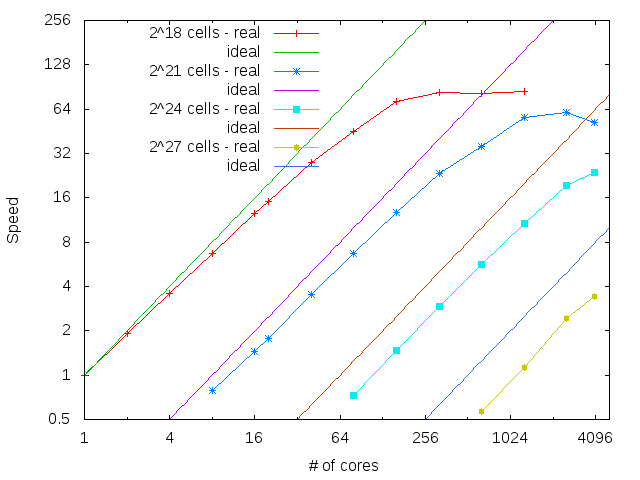
\includegraphics[scale=0.75]{./scaling.png}
\caption{Scaling of Octo-Tiger on SuperMIC - Depicted are time-steps per wall clock time vs. number of processing cores for Octo-Tiger using four problem sizes. 
The results are normalized such that the single processor run for the smallest problem has a speed of $1$. We also
show lines corresponding to ideal strong and weak scaling for each problem size, with the same normalization. }
\label{scaling}
\end{figure}


\section{Research Plan}

 We would like to run at least two DWD models. The first will be an equal mass binary and it is not expected to merger. This will be for testing purposes, to ensure Octo-Tiger delivers results that are
consistent with physical expectations, and  to ensure Octo-Tiger conserves
momenta and energy to machine precision. Next, we will drive an unequal mass semi-detched binary to merger. The merged remannt will then be investigated using other codes that do not require HPC. 
Each run should take about 20 orbits each. For each run we would like to use two problem sizes, one of 2\^24 and 2\^27 cells. Because our application scales well we will use 200 nodes for each run.



\section{Requirements}
The wall clock 
time required for one timestep is approximately 0.5 and 4 seconds, respectively. Although we have a good idea of how fast Octo-Tiger executes in terms of the wallclock time required for one timestep, it is 
difficult to predict the number of required timesteps ahead of time. Initial tests suggest the required number of timesteps per orbit for the 2\^24 cell and 2\^27 cell problems is 16,000 and 32,000 steps, 
respectively. The total number of SU's required for these runs is therefore 2 runs X 32,000 timesteps per orbit X 4 seconds per timestep X 20 orbits X 128 nodes X 20 cores + 2 runs X 16,000 timesteps per 
orbit X 0.5 seconds per timestep X 20 orbits X 128 nodes X 20 cores =  3,640,888 SUs + 227,555 SUs = 3,868,443 SUs. 

We will also be experimenting with an N-body gravity code. This code will require 8 nodes for about 10 hours for each execution, and we would like to execute the code around one hundred times. The SU requirement for 
this portion of our request is 8 nodes X 20 cores X 10 hours X 100 = 160,000 SUs.

Our total SU requirement is 3,868,443 SUs  + 160,000 SUs =  4028443 SUs.  Because the maximum amount of time allowed for a request is 3,000,000, we are requesting 3,000,000 SUs. 

\bibliography{mike}


 \end{document}

